\chapter{PHƯƠNG PHÁP THỰC HIỆN}\label{Chapter3}

\section*{Tóm tắt chương}

Chương này trình bày thiết kế hệ thống học chắt lọc liên kết tích hợp học tiệm tiến cho phát hiện xâm nhập mạng. Nội dung gồm kiến trúc tổng thể, luồng dữ liệu, vai trò client, cơ chế chắt lọc, vòng học tiệm tiến và các cấu hình thuật toán.

\section{Yêu cầu bài toán}

Hệ thống cần đáp ứng bốn yêu cầu chính:

\begin{itemize}
    \item Thứ nhất, client không được chia sẻ dữ liệu huấn luyện hoặc trọng số mô hình.
    \item Thứ hai, hệ thống phải học được từ dữ liệu Non-IID và mất cân bằng lớp.
    \item Thứ ba, hệ thống hỗ trợ học thêm lớp tấn công mới theo từng tác vụ.
    \item Thứ tư, cơ chế truyền tri thức không phụ thuộc tuyệt đối vào việc mọi client dùng cùng kiến trúc mô hình.
\end{itemize}

\section{Hệ thống đề xuất}

\subsection{Mô tả tổng quan hệ thống đề xuất}

Hệ thống đề xuất hướng đến bài toán phát hiện xâm nhập trong môi trường học phân tán, nơi dữ liệu giữa các client không đồng nhất, các lớp tấn công mới xuất hiện theo thời gian và việc trao đổi dữ liệu riêng hoặc trọng số mô hình không phù hợp với yêu cầu vận hành. Thay vì tổng hợp tham số như các phương pháp FL truyền thống, hệ thống tổ chức quá trình cộng tác thông qua FD: mỗi client huấn luyện mô hình cục bộ trên dữ liệu riêng, sinh logits trên tập dữ liệu public (dữ liệu công khai không gán nhãn) và gửi các tập logits này cho phần tử điều phối để tạo consensus logits.

Đầu tiên, hệ thống giả định ở mỗi task học tiệm tiến $t$, có tổng cộng $|K|$ client tham gia học liên kết. Ở mỗi client tồn tại dữ liệu huấn luyện riêng $D_k$ và mô hình phân loại $f_k$. Các client đều có thể truy cập một bộ dữ liệu công khai không nhãn $D_p$, bộ dữ liệu replay của tác vụ cũ gồm bộ đặc trưng $\mathcal X$ và nhãn giả tương ứng $\mathcal Y$, cũng như bộ logit $\mathcal Z$ của các mẫu replay đó. Mỗi client huấn luyện giám sát mô hình $f_k$ trên tập dữ liệu riêng kết hợp với tập dữ liệu replay $D_k \cup {\mathcal X; \mathcal Y}$. Sau đó, mỗi mô hình $f_k$ dự đoán tập logit $z_k^t$ của bộ dữ liệu public ở task hiện tại $D_p^t$. Bên cạnh đó, để cập nhật số chiều của logit $\mathcal Z$ của mẫu dữ liệu public thuộc task cũ, từng client cũng sinh thêm biểu diễn logit mới $\mathcal Z_k$.

Từ phân phối logit trên dữ liệu riêng $D_k$, mỗi client $k$ tính ra phân phối energy của riêng nó $E(x) \forall x \in D_k$, và chọn ra phân vị thứ $q$ để làm ngưỡng lọc $\tau_k^t$. Từ ngưỡng này, mỗi client tự tạo một mặt nạ binary $m_k^t$ để đánh dấu các dự đoán logit trên tập công khai, trong đó $m_k^t(x) = 0$ có nghĩa mẫu $x$ không nằm trong phân phối dữ liệu của $D_k$, và $1$ có nghĩa ngược lại.

Từng client gửi bộ logit dự đoán $z_k^t \cup \mathcal Z_k$ cho phần tử client điều hướng. Client điều hướng thực hiện tổng hợp logit sử dụng thuật toán Robust Logit Fusion và tạo ra bộ logit tổng hợp $\bar z \leftarrow \bar z^t \cup \mathcal Z$ và truyền $\bar z$ cho mọi client. Trong đó, các logit $\mathcal Z$ chỉ được trả về nếu argmax của nó trung với nhãn giả $\mathcal Y$ tương ứng.

Nếu vòng liên kết là vòng cuối cùng của task $t$, client điều phối thực hiện argmax ra nhãn giả của các mẫu dữ liệu task hiện tại $D_p^t$. Với mỗi lớp, client điều phối tính ra trung tâm của lớp $\mu_c^t$ và chọn một tỉ lệ mẫu dữ liệu replay xung quanh trung tâm này. Các mẫu public được chọn $\mathcal X^t$ cùng nhãn giả tương ứng $\mathcal Y^t$ được thêm vào bộ dữ liệu replay $\mathcal X, \mathcal Y$ Ở bước Robust Logit Fusion, dựa trên tỉ lệ bị loại của dự đoán mà từng client $k$ được chấm điểm outlier $\rho_k^t$. Client có số điểm outlier thấp nhất trở thành client điều phối của vòng liên kết tiếp theo.

Sau cùng, bộ logit của task hiện tại và bộ logit tái diễn được trả về cho toàn bộ client. Từng client tự học chắt lọc sử dụng kỹ thuật Evidential Knowledge Distillation để cập nhật mô hình $f_k$ của riêng nó.

\subsection{Quy trình hoạt động chi tiết}

\begin{figure*}[ht]
    \centering
    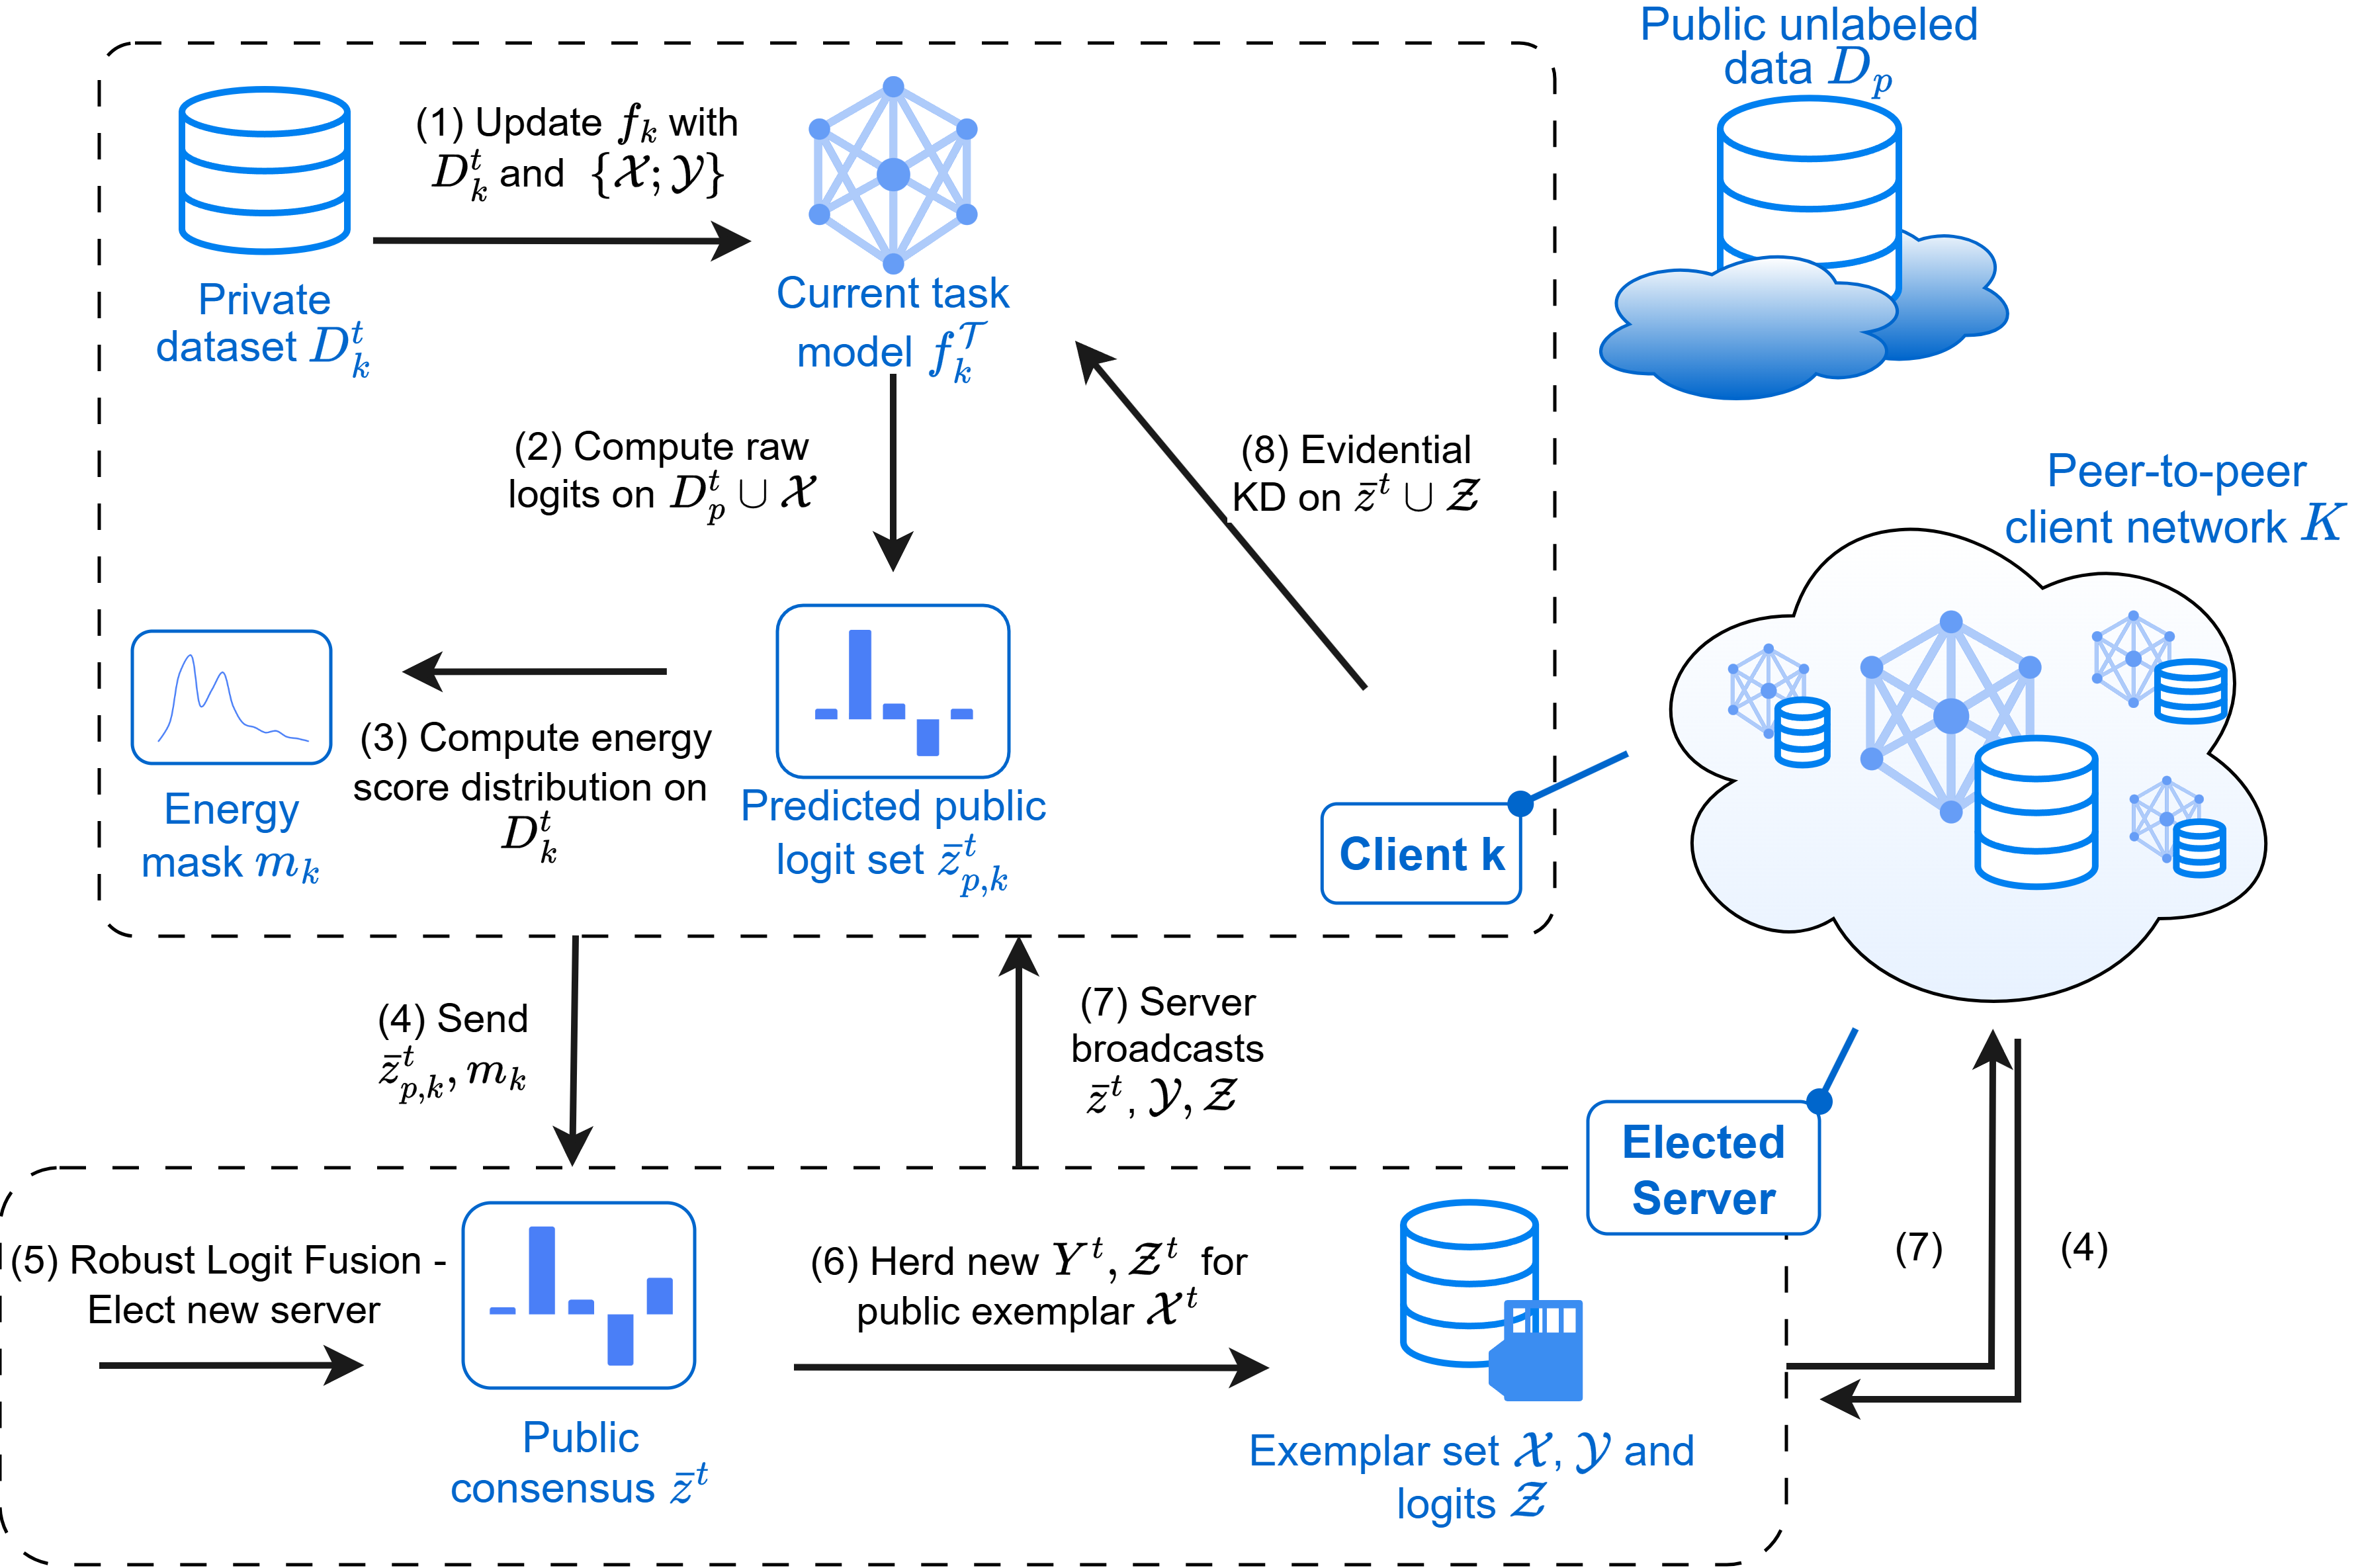
\includegraphics[width=1.0\textwidth]{images/FCIL_ours3.png}
    \caption{Kiến trúc khái quát của phương pháp đề xuất.}
    \label{fig:pipeline}
\end{figure*}

Hình \ref{fig:pipeline} minh họa quy trình hoạt động của hệ thống đề xuất. Thuật toán \ref{alg:proposed_fd_cil_flow} được đặt ngay sau sơ đồ để làm điểm tham chiếu chính; các bước 1--8 trong thuật toán đi theo đúng thứ tự trong hình, và các công thức đi kèm được đánh số để có thể được dẫn chiếu trực tiếp trong phần diễn giải.

\begin{algorithm}[H]
    \LinesNumbered
    \newcommand{\algwrap}[2][1]{\parbox[t]{\dimexpr\linewidth-#1\algomargin-1.5em\relax}{\raggedright#2}}
    \KwInput{\algwrap[3]{Chuỗi task $\{\mathcal{T}_t\}_{t=1}^{T}$, tập client theo task $K_t$, dữ liệu riêng $D_k^t$, tập public $D_p^t$, số vòng $R_t$, quantile energy $q$, ngưỡng robust $\theta$, tỉ lệ nhớ $m$}}
    \KwOutput{\algwrap[3]{Các mô hình cục bộ cuối $\{w_k^T\}$ cùng $\mathcal X^T$, $\mathcal Y^T$, $\mathcal Z^T$}}
    $\mathcal X^0\gets\emptyset$, $\mathcal Y^0\gets\emptyset$, $\mathcal Z^0\gets\emptyset$\;
    Chọn ngẫu nhiên client điều phối đầu tiên từ $K_1$\;
    \For{$t\gets1$ \KwTo $T$}{
        Mở rộng classifier head theo tập lớp mới của $\mathcal{T}_t$\;
        \For{$r\gets1$ \KwTo $R_t$}{
            \ForEach{client $k\in K_t$}{
                \textbf{1.} Cập nhật $f_k$ với $D_k^t$ và $(\mathcal X^{<t},\mathcal Y^{<t})$\;
                \textbf{2.} Tính raw logits $z_{p,k}^t$ trên $D_p^t\cup\mathcal X^{<t}$\;
                \textbf{3.} Tính phân phối energy trên $D_k^t$ và tạo mặt nạ $m_k^t$\;
                \textbf{4.} Gửi $(z_{p,k}^t,m_k^t)$ cho client điều phối\;
            }
            \ForEach{$x\in D_p^t$}{
                \textbf{5.} Robust Logit Fusion trên $\{z_k^t(x)\mid k\in K_t\}$, tính consensus $\bar z^t(x)$ và chọn client điều phối mới\;
            }
            \ForEach{$x\in\mathcal X^{<t}$}{
                Tính consensus replay mới và giữ lại logits hợp lệ trong $\mathcal Z$ nếu nhãn dự đoán khớp $\mathcal Y$\;
            }
            \If{$r=R_t$}{
                \ForEach{pseudo class $c$ từ $\hat y^t(x)=\arg\max_c\bar z_c^t(x)$ trên $D_p^t$}{
                    \textbf{6.} Herd nhãn giả $\mathcal Y^t$, logits $\mathcal Z^t$ và public exemplar $\mathcal X^t$\;
                }
            }
            \textbf{7.} Client điều phối broadcast $\bar z^t$, $\mathcal Y$ và $\mathcal Z$ cho các client\;
            \ForEach{client $k\in K_t$}{
                \textbf{8.} Chắt lọc EKD trên $\bar z^t\cup\mathcal Z$ để cập nhật $f_k$\;
            }
        }
    }
    \Return $\{w_k^T\}$, $\mathcal X^T$, $\mathcal Y^T$, $\mathcal Z^T$\;
    \caption{Luồng hoạt động FD-CIL của phương pháp đề xuất với replay public}
    \label{alg:proposed_fd_cil_flow}
\end{algorithm}

Trước khi đi vào bước 1 của Thuật toán \ref{alg:proposed_fd_cil_flow}, hệ thống xác định tập lớp mới của task hiện tại, tập client tham gia, dữ liệu riêng của từng client và tập public dùng làm bề mặt chung để trao đổi tri thức. Tại task $t$, mỗi client $k\in K_t$ sở hữu dữ liệu riêng $D_k^t$, trong khi toàn hệ thống cùng dùng tập public không gán nhãn $D_p^t$ để trao đổi tri thức ở mức logits. Mô hình cục bộ của client được ký hiệu là $f_k^t$, và logit trước softmax của client $k$ trên mẫu $x$ được ký hiệu là $z_k^t(x)$. Ký hiệu logits được giữ xuyên suốt chương này vì cơ chế EVA, Robust Logit Fusion và EKD đều khai thác độ lớn của logits thay vì dùng xác suất sau softmax.

\subsubsection{Trạng thái dữ liệu và bộ nhớ dữ liệu tái diễn}

Trong học tiệm tiến, nếu client chỉ học dữ liệu của task mới, mô hình dễ dịch chuyển khỏi những lớp đã học ở các task trước (catastrophic forgetting). Tuy nhiên, lưu lại dữ liệu riêng của client cũ không phù hợp với ràng buộc phân tán và quyền riêng tư của hệ thống. Vì vậy, phương pháp đề xuất sử dụng học tiệm tiến dựa trên replay đến từ các mẫu public $x \in D_p$, trong đó những mẫu được giữ lại $\mathcal X$ đều lấy từ tập public $D_p$ thay vì lấy từ dữ liệu riêng. Bộ nhớ replay gồm ba thành phần: $\mathcal X$ lưu các mẫu dữ liệu không nhãn đã chọn để replay, $\mathcal Y$ lưu nhãn cứng tính từ bộ consensus tương ứng, còn $\mathcal Z$ lưu phần logits exemplar hợp lệ dùng làm tín hiệu mềm trong EKD. Trong ba thành phần này, $\mathcal Y$ chỉ được mở rộng ở cuối task, trong khi $\mathcal Z$ được làm mới liên tục ở từng vòng liên kết và kiểm tra lại ở các task sau trước khi tham gia chắt lọc. Bên cạnh đó, các mô hình khi chuyển sang một tác vụ mới cần phải mở rộng đầu ra của lớp phân loại. Đây là một đặc điểm của học tiệm tiến dựa trên dynamic architecture. Thay vì trực tiếp chắt lọc phân phối của mô hình cũ cho mô hình mới, phương pháp đề xuất chắt lọc tri thức chung của các client sau bước học replay cho mô hình mới, kết hợp học liên kết và học tiệm tiến trong cùng một bước chiết xuất.

\subsubsection{Bước 1: Cập nhật mô hình cục bộ bằng dữ liệu hiện tại và tái diễn dữ liệu}

Ở bước 1, client cần cập nhật $f_k$ bằng dữ liệu hiện tại nhưng vẫn được nhắc lại các lớp cũ. Với task đầu tiên, bộ nhớ replay rỗng nên client chỉ tối ưu trên dữ liệu riêng $D_k$ hiện tại. Từ task thứ hai trở đi, đầu ra phân loại của mô hình được mở rộng để cùng chiều với tổng số nhãn (cũ và mới), trong khi dữ liệu huấn luyện cục bộ được tạo bằng cách ghép dữ liệu riêng của task mới với các public exemplars cũ $D_k \cup \mathcal X$ đã có nhãn cứng $\mathcal Y$:
\begin{equation}
\label{eq:local_replay_dataset}
	\tilde D_k^t=D_k^t\cup(\mathcal X^{<t},\mathcal Y^{<t}).
\end{equation}
Với mẫu $(x,y)\in\tilde D_k^t$, client tối ưu hàm mất mát cross-entropy có giám sát:
\begin{equation}
\label{eq:local_ce_loss}
L_{local,k}^t=\frac{1}{|\tilde D_k^t|}\sum_{(x,y)\in\tilde D_k^t}CE(y,p_k^t(x)),
\qquad p_k^t(x)=\operatorname{softmax}(z_k^t(x)).
\end{equation}
Cách ghép trong công thức \ref{eq:local_replay_dataset} đặt quá trình replay ngay trong bước 1, nên CIL không còn là một cơ chế tách rời sau FD. Lớp mới được học từ dữ liệu riêng có nhãn thật, còn lớp cũ được nhắc lại bằng public exemplars đã được consensus gán nhãn ở các task trước thông qua hàm mục tiêu trong công thức \ref{eq:local_ce_loss}. Sau khi cập nhật cục bộ, bước 2 yêu cầu client sinh raw logits $z_{p,k}^t$ trên $D_p^t\cup\mathcal X^{<t}$, nhờ đó task hiện tại và replay features cũ cùng đi vào không gian dự đoán chung trước khi được lọc và tổng hợp.

\subsubsection{Bước 2: Sinh logits cho dữ liệu công khai}

Sau khi đã học giám sát kết hợp học tiệm tiến replay ở bước 1, hệ thống cần cập nhật các mẫu logit replay của các mẫu replay public, vì số chiều của logit đã tăng lên theo số lớp. Như vậy, bên cạnh việc dự đoán logit cho các mẫu public thuộc task hiện $D_p^t$, các mô hình còn cần dự đoán cả các mẫu exemplar $\mathcal X$ trên tập dữ liệu public từ task trước. Sau bước 2, ở mỗi client đã tồn tại tập dự đoán $z \leftarrow \bar z_{p,k}^t \cup \mathcal Z_k$, trong đó $\bar z_{p,k}^t$ là phân phối logit của tập dữ liệu public ở tác vụ $t$ của mô hình thuộc client $k$, cũng như $\mathcal Z_k$ là phân phối logit của dữ liệu replay của tất cả các tác vụ trước do mô hình $f_k$ dự đoán.

\subsubsection{Bước 3: Sinh phân phối energy và chọn ngưỡng lọc trong EVA}

Tập public giúp các client gặp nhau ở cùng một không gian dự đoán, nhưng không phải public sample nào cũng nằm gần phân phối riêng của mọi client. Nếu mọi client đều đóng góp logits với cùng mức tin cậy, consensus có thể bị kéo lệch bởi những dự đoán thiếu cơ sở. Vì vậy, EVA được đưa vào để mỗi client tự đánh giá public sample nào thuộc gần phân phối dữ liệu riêng của mình thành trọng số tổng hợp đi kèm dự đoán để logits được tổng hợp ổn định hơn.

Phát hiện ngoài phân phối bằng energy (Energy-based Out-of-distribution detection) xuất phát từ nhận xét rằng xác suất softmax lớn nhất của mô hình thường quá tự tin ngay cả với mẫu ngoài phân phối, vì softmax không nhạy với phép dịch trên logit \cite{liu2020energy}. Với logit $z_i$ và temperature $T$, energy của mẫu $x$ được định nghĩa là
\begin{equation}
\label{eq:energy_general}
E(x) = -T\log\sum_i e^{z_i/T}.
\end{equation}
Giá trị energy thấp thường đi với mẫu nằm trong phân phối huấn luyện, vì mô hình tạo ra một hoặc nhiều logit có độ lớn đủ cao để kéo giá trị log-sum-exp lên. Ngược lại, giá trị energy cao cho thấy các giá trị logit thường trải đều và thấp, nên các mẫu với energy cao có khả năng thuộc vùng ngoài phân phối. Trong IDS, cách nhìn này hữu ích vì lưu lượng mới, biến thể tấn công mới hoặc mẫu bị nhiễu không nhất thiết tạo ra xác suất softmax thấp, nhưng vẫn có thể biểu hiện qua energy cao hơn so với các mẫu quen thuộc.

Ở bước 3, với logit $z_k^t(x)$, energy của client $k$ được tính bằng
\begin{equation}
\label{eq:client_energy}
E_k^t(x)=-T\log\sum_i\exp(z_{k,i}^t(x)/T).
\end{equation}
Ngưỡng lọc của client được ước lượng từ phân phối energy trên dữ liệu riêng hiện tại:
\begin{equation}
\label{eq:eva_threshold}
\tau_k^t=Q_q(\{E_k^t(x)\mid x\in D_k^t\}).
\end{equation}
Sau đó, client sinh logits trên cả public samples của task hiện tại và replay features cũ, rồi tạo mặt nạ EVA:
\begin{equation}
\label{eq:eva_mask}
m_k^t(x)=\mathbb{I}[E_k^t(x)\leq\tau_k^t],\qquad x\in D_p^t\cup\mathcal X^{<t}.
\end{equation}
Ở bước 4, client gửi cặp $(z_k^t(x),m_k^t(x))$ cho phần tử điều phối. Nhờ mặt nạ trong công thức \ref{eq:eva_mask}, dự đoán có energy cao vẫn có thể được ghi nhận, nhưng không được xem là đóng góp đáng tin trong bước logit fusion.

\subsection{Bước 4: Client cập nhật phân phối logit và mặt nạ EVA lên phần tử điều phối}

Sau khi tất cả các client đã hoàn thành bước 3, ở mỗi client $k \in K^t$ tham gia vòng liên kết đó đã tồn tại bộ logit dự đoán cho tập dữ liệu public $\bar z_{p,k}^t$ và tập replay public $\mathcal Z_k$, cũng như mặt nạ EVA cho cả hai tập logit này $m_k$. Toàn bộ client upload các dữ liệu này về client đảm nhiệm vai trò điều phối để tiến hành tổng hợp.

\subsubsection{Bước 5: Robust Logit Fusion và lựa chọn phần tử điều phối}

EVA làm giảm ảnh hưởng của những dự đoán nằm ngoài phân phối riêng của từng client, nhưng trong tập logits gửi về vẫn có thể tồn tại những vector quá lệch so với phần còn lại do Non-IID, kéo giá trị tổng hợp theo hướng bất lợi. Vì vậy, Blom Robust Filter được dùng như tầng làm sạch thứ hai trước khi tổng hợp consensus sau cùng.

Cụ thể, ở bước 5, với tập client đang hoạt động $K^a$, hệ thống tính trung bình và covariance của các logits, lấy eigenvector cao nhất $v(x)$, rồi ánh xạ từng logit lên hướng này:
\begin{equation}
\label{eq:robust_projection}
s_k^t(x)=v(x)^\top(z_k^t(x)-\bar z^{a,t}(x)),\qquad k\in K^a.
\end{equation}
Median projection và thang đo MAD được tính bằng
\begin{equation}
\label{eq:robust_mad}
\tilde s^t(x)=\operatorname{median}_{k\in K^a}s_k^t(x),
\qquad
\sigma^t(x)=1.4826\cdot\operatorname{median}_{k\in K^a}|s_k^t(x)-\tilde s^t(x)|.
\end{equation}
Độ lệch chuẩn hóa của client là
\begin{equation}
\label{eq:robust_distance}
d_k^t(x)=\frac{|s_k^t(x)-\tilde s^t(x)|}{\sigma^t(x)}.
\end{equation}
Các giá trị này được so sánh với ngưỡng Blom theo rank để tạo mặt nạ outlier $o_k^t(x)$. Sau khi có mặt nạ outlier và mặt nạ EVA, consensus trên public sample hiện tại được tính bằng
\begin{equation}
\label{eq:consensus_logit}
\bar z^t(x)=\frac{\sum_{k\in K_t}m_k^t(x)(1-o_k^t(x))z_k^t(x)}{\sum_{k\in K_t}m_k^t(x)(1-o_k^t(x))},\qquad x\in D_p^t.
\end{equation}
Tỉ lệ bị loại của từng client được tính trên tập public:
\begin{equation}
\label{eq:filter_score}
\rho_k^t=\frac{1}{|D_p^t|}\sum_{x\in D_p^t}o_k^t(x).
\end{equation}
Client có $\rho_k^t$ thấp hơn cho thấy logits của nó ít bị xem là outlier hơn, nên hệ thống chọn phần tử điều phối của vòng tiếp theo từ các client có filter score $\rho_k^t$ thấp nhất ngay trong bước 5. Nhờ vậy, cơ chế điều phối vẫn giữ bản chất phi tập trung nhưng ưu tiên client đang tạo tri thức ổn định hơn.

\subsubsection{Bước 6: Cập nhật dữ liệu tái diễn}

Sau bước 5, mẫu replay từ tập dữ liệu public cũ không chỉ tham gia học giám sát cross-entropy, mà còn tham gia vào giai đoạn chắt lọc ở sau bước tổng hợp. Tuy nhiên, logits mềm cũ không tương thích trực tiếp, vì không gian lớp đã mở rộng sau mỗi task. Do đó, với mỗi mẫu cũ $x\in\mathcal X^{<t}$, client sinh lại logits sử dụng mô hình $f_k$ sau bước học giám sát trên $D_k \cup \{\mathcal X, \mathcal Y\}$ hiện tại. Phần tử điều phối tổng hợp các logit đã cập nhật số chiều này song song với logit của task hiện tại, rồi tạo consensus replay mới $\mathcal Z$ để chuẩn bị cho bước broadcast.

Nếu bước này xảy ra trong vòng liên kết cuối cùng của task, hệ thống cần herd một phần dữ liệu public của tác vụ hiện tại để phục vụ quá trình học tiệm tiến replay các task sau. Việc lưu toàn bộ public là không cần thiết và làm tăng chi phí replay, nên phương pháp đề xuất chỉ giữ những mẫu có consensus logits gần trung tâm của từng pseudo class. Với consensus $\bar z$ trên $D_p^t$, nhãn cứng của public sample được xác định bằng
\begin{equation}
\label{eq:pseudo_label}
\hat y^t(x)=\arg\max_c\bar z_c^t(x).
\end{equation}
Các mẫu được gom theo pseudo class:
\begin{equation}
\label{eq:pseudo_group}
G_c^t=\{x\in D_p^t\mid \hat y^t(x)=c\},
\qquad
\mu_c^t=\frac{1}{|G_c^t|}\sum_{x\in G_c^t}\bar z^t(x).
\end{equation}
Với mỗi lớp giả $c$, hệ thống chọn $m\%$ mẫu có logit gần $\mu_c^t$ nhất:
\begin{equation}
\label{eq:exemplar_select}
\mathcal X_c^t=\operatorname{TopClose}_{m\%}\{x\in G_c^t;\|\bar z^t(x)-\mu_c^t\|_2\}.
\end{equation}
Bộ nhớ replay được mở rộng ở cuối task bằng
\begin{equation}
\label{eq:memory_update_xy}
\mathcal X^t=\mathcal X^{<t}\cup\bigcup_c\mathcal X_c^t,
\qquad
\mathcal Y^t=\mathcal Y^{<t}\cup\bigcup_c\{\hat y^t(x)\mid x\in\mathcal X_c^t\},
\end{equation}
\begin{equation}
\label{eq:memory_update_z}
\mathcal Z^t=\mathcal Z^{<t}\cup\bigcup_c\{\bar z^t(x)\mid x\in\mathcal X_c^t\}.
\end{equation}
$\mathcal Y$ được nối thêm một lần cho task hiện tại, còn $\mathcal Z$ lưu consensus tại thời điểm chọn mẫu nhưng vẫn sẽ được làm mới và kiểm chứng lại khi replay xuất hiện trong task sau.

Bộ logit replay chỉ được chấp nhận nếu nhãn dự đoán của nó vẫn khớp với nhãn $\mathcal Y$:
\begin{equation}
\label{eq:replay_consistency}
\arg\max_c\mathcal Z_c(x)=y_x,\qquad y_x\in\mathcal Y^{<t}.
\end{equation}
Điều này làm rõ vai trò khác nhau của $\mathcal Y$ và $\mathcal Z$. Tập $\mathcal Y$ là tập nhãn cứng không đổi theo thời gian, chỉ được nối thêm ở cuối các task và không bị sửa lại ở các vòng sau. Ngược lại, $\mathcal Z$ được cập nhật liên tục: nó được làm mới từ $\mathcal X$ dưới không gian lớp hiện tại, sau đó bị lọc bằng $\mathcal Y$. Vì vậy, số logits hợp lệ trong $\mathcal Z$ ở một vòng có thể nhỏ hơn số nhãn đang được lưu trong $\mathcal Y$.

\subsubsection{Bước 7: Cập nhật bộ logit tổng hợp và nhãn cứng cho học tái diễn}

Sau khi tổng hợp, phần tử điều phối broadcast bộ dữ liệu replay gồm đặc trưng $\mathcal X$ và logits hợp lệ $\mathcal Z$ cũng như bộ logit của tác vụ hiện tại $\bar z^t$ trên dữ liệu public cho mọi client tham gia. Như đã giải thích ở bước 6, logits replay và logits của tác vụ hiện tại luôn được cập nhật và trả về ở mỗi vòng liên kết, trong khi bộ nhãn cứng replay chỉ được cập nhật và thêm mới ở cuối task $t$. Do đó, phần tử điều phối cũng broadcast kèm bộ nhãn replay $\mathcal Y$ đã cập nhật ở vòng liên kết cuối cùng mỗi task.

\subsubsection{Bước 8: Evidential Knowledge Distillation}

Ở bước 8, sau khi có consensus trên $D_p^t$ và phần replay logits hợp lệ $\mathcal Z$, phần tử điều phối broadcast teacher logits $\bar z^t(x)$, nhãn giả $\mathcal Y$ và logits replay $\mathcal Z$ về các client. Mục tiêu của bước 8 là đưa tri thức đã được tổng hợp quay lại toàn bộ client tham gia, nhưng vẫn không yêu cầu trao đổi trọng số mô hình. Phương pháp đề xuất dùng EKD vì logits không chỉ chứa thứ tự ưu tiên giữa các lớp, mà còn phản ánh mức bằng chứng và độ chắc chắn của consensus.

Với teacher logit $\bar z^t(x)$ và student logit $z_k^t(x)$ từ các mẫu public $x \in D_p$, tham số Dirichlet được tạo bằng
\begin{equation}
\label{eq:dirichlet_evidence}
\alpha^T(x)=\exp(\bar z(x))+\lambda_{prior},
\qquad
\alpha_k^S(x)=\exp(z_k(x))+\lambda_{prior}.
\end{equation}
Mất mát EKD gồm tầng căn chỉnh tỷ lệ bằng chứng và tầng căn chỉnh toàn bộ phân phối Dirichlet:
\begin{equation}
\label{eq:ekd_loss}
L_{EKD,k}^t=L_{1st,k}^t+\gamma L_{2nd,k}^t.
\end{equation}
Bước chắt lọc này tách hẳn khỏi giai đoạn học giám sát trước đó, nên mỗi vòng huấn luyện của client được chia thành hai pha tuần tự thay vì gộp chung vào một hàm mất mát duy nhất. Ở pha thứ nhất, client tối ưu riêng mục tiêu giám sát $L_{local,k}^t$ trên dữ liệu riêng cùng nhãn cứng trong quá trình replay, qua đó học các lớp mới và củng cố tri thức cũ:
\begin{equation}
\label{eq:local_update}
\theta_k^{t,\,\text{(1)}}\leftarrow\arg\min_{\theta_k}L_{local,k}^t.
\end{equation}
Sau bước 7, khi đã có được bộ logit từ nhãn công khai hiện tại và replay, từng client tối ưu mục tiêu chắt lọc $L_{EKD,k}^t$ trên kiến thức chắt lọc từ mô hình teacher $\bar z$ tại $D_p^t \cup \mathcal X$:
\begin{equation}
\label{eq:ekd_update}
\theta_k^{t,\,\text{(2)}}\leftarrow\arg\min_{\theta_k}L_{EKD,k}^t.
\end{equation}

\subsection{Mô hình phát hiện xâm nhập}

\subsubsection{Đơn mô hình}

Trong thiết lập đơn mô hình, toàn bộ client sử dụng cùng một kiến trúc phát hiện xâm nhập, cùng số chiều đầu ra và cùng cách biểu diễn tham số. Thiết lập này phù hợp với các phương pháp FL dựa trên tổng hợp trọng số vì mô hình của mọi client có cùng cấu trúc, nên server hoặc phần tử điều phối có thể cộng trung bình tham số theo từng lớp. Tuy nhiên, ràng buộc đồng nhất kiến trúc làm giảm tính linh hoạt của hệ thống khi các client có tài nguyên tính toán, kiểu lưu lượng mạng hoặc yêu cầu triển khai khác nhau.

\subsubsection{Đa mô hình}

Trong thiết lập đa mô hình, các client có thể sử dụng các kiến trúc phát hiện xâm nhập khác nhau, chẳng hạn mô hình tuần tự, mô hình tích chập hoặc mô hình lai, miễn là chúng cùng ánh xạ dữ liệu đầu vào về không gian nhãn chung của bài toán. Phương pháp đề xuất hoàn toàn tương thích với thiết lập này vì quá trình cộng tác diễn ra trên logits thay vì trên trọng số mô hình. Mặt khác, energy sinh ra trong bước EVA hoàn toàn phụ thuộc vào từng kiến trúc và phân phối dữ liệu riêng của client, và Robust Logit Fusion cũng như EKD trong Thuật toán \ref{alg:proposed_fd_cil_flow} chỉ yêu cầu các client sử dụng chung số chiều của lớp dự đoán đầu ra (logit layer), một điều kiện hoàn toàn bình thường trong học liên kết.

\section{Đầu ra của hệ thống}

Hệ thống tạo log huấn luyện, file kết quả theo vòng, bản ghi trọng số của mô hình toàn cục hoặc trọng số client theo vòng và các bảng đánh giá cuối. Các đầu ra này phục vụ phân tích hiệu năng, so sánh thuật toán và tái đánh giá.
